\subsection{Adjustable Positive Voltage Regulator:}

In this section we analyze a {\bfseries\itshape Adjustable Positive Voltage Regulator}. The IC that we use was the {\bfseries\itshape LM317}. Following the Figure 3.4.0, we assembled the circuit, and this time, we used a fixed voltage source $V_{in}$ = 20 V. What we are going to adjust it's the resistor $R_{2}$, this resistor it's a potentiometer of 10k$\Omega$ max:

\begin{figure}[H]
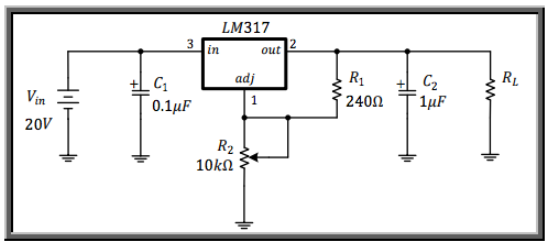
\includegraphics[scale=.6]{d4.png}
\centering \linebreak \linebreak Figure 3.4.0: Adjustable positive voltage regulator circuit.
\end{figure}

Once the circuit were assembled, we put the potentiometer in his minimum and maximum resistance, and measure the voltage in the resistor $R_{L}$ in each case, $V_{0_{min}}$ and $V_{0_{max}}$ respectively: \hfill \break

{\bfseries\itshape\color{armygreen}{Observation:}} {\itshape\color{armygreen}{For measure the voltage in $R_{L}$ it's necessary to connect a voltmeter in parallel with the resistor.}} \hfill

\begin{ceqn}
\begin{align}
V_{0_{max}} = 18.2 V \\
V_{0_{min}} = 1.2 V
\end{align}
\end{ceqn}

\pagebreak